\documentclass{article}
\usepackage{amsmath}
\usepackage{mathtext}
\usepackage[english,russian]{babel}
\usepackage[T2A]{fontenc}
\usepackage[utf8]{inputenc}
\usepackage{graphicx}
\graphicspath{{img/}}
\DeclareGraphicsExtensions{.jpg, .pdf}
\begin{document}
\section{Сложные передачи. Рядные передачи. Ступенчатые передачи}

\underline{Рядные передачи}

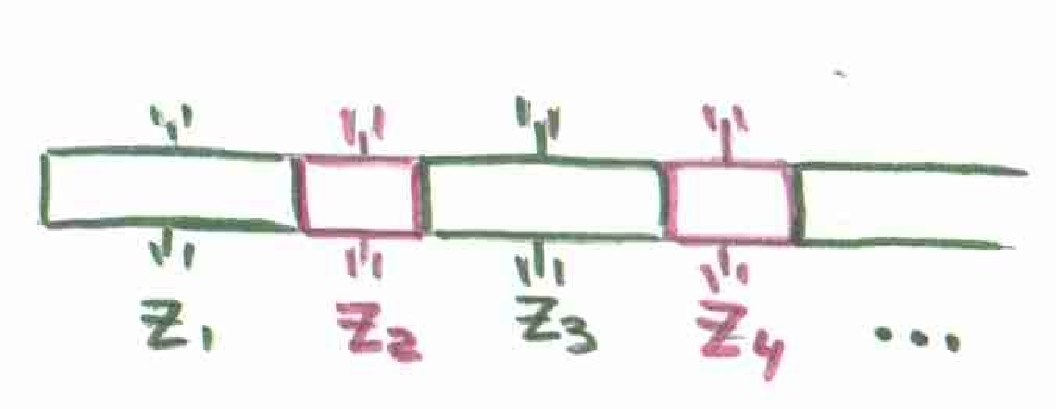
\includegraphics[width = 0.75\textwidth]{1}

$n$ -- количество зубчатых колес\\
$k$ -- количество зацеплений\\
$i_{1n} = (-1)^k \frac{z_n}{z_1}$\\
$\eta = \eta_{1\:2}\cdot\eta_{2\:3}\cdot\dots\cdot\eta_{i\:j}$\\
\underline{Применение:}
\begin{enumerate}
	\item Позволяют вписывать передачу в занные межосевые расстояния
	\item Когда необходимо согласовать вращение входного и выходного вала
	\item Служат для обхода препятствий внутри конструкций
\end{enumerate}
\underline{Достоинства:} 
\begin{enumerate}
	\item Возможность согласования валов на определенном межосевом расстоянии
	\item Возможность смены навпрления вращения передачи без пересчета передаточного отношения
	\item Возможноность обходения препятствий внутри конструкции
	\item Возможность снятия показаний с нескольких выходных валов
\end{enumerate}
\underline{недостатки:} 
\begin{enumerate}
	\item В передаточном отношении участвуют только первое и последнее зубчатые колеса, все остальные являются паразитными
	\item Относительно низкое КПД
	\item Большое кол-во промежуточных элементов
\end{enumerate}

\underline{Многоступенчатые передачи} 

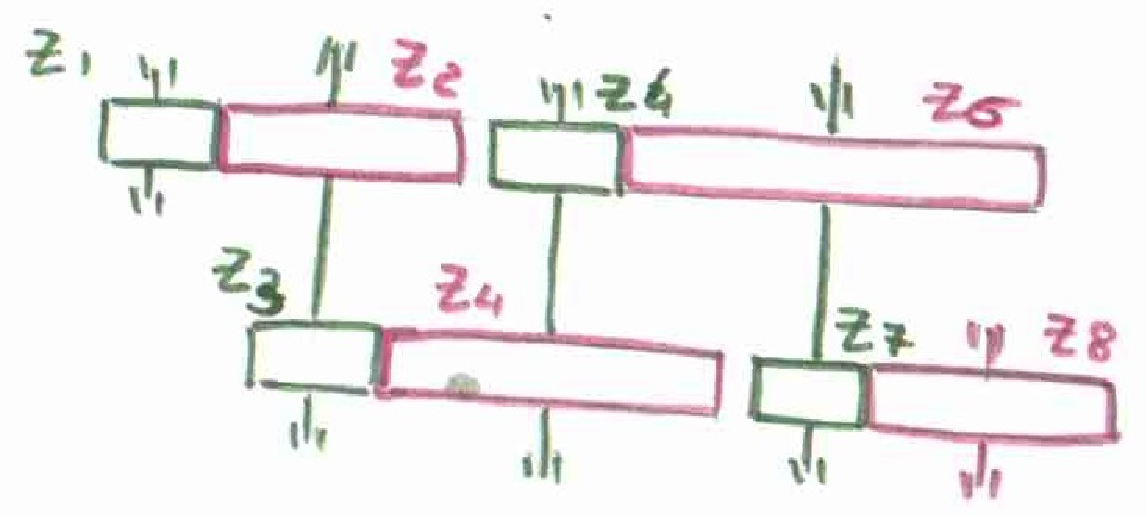
\includegraphics[width = 0.75\textwidth]{2}

$i_{1n} = (-1)^k \frac{z_2 \dots z_n}{z_1 \dots z_{n-1}} = i_{12} \cdot i_{34} \cdot \dots \cdot i_{(n-1)n}$\\
$\eta = \eta_{12} \cdot \eta_{34} \cdot \dots \cdot \eta_{(n-1)n}$\\
\underline{Применяются}, когда необходимо получить высокое пердаточное отношение
\underline{Достоинства:}
\begin{enumerate}
	\item Можно получить как очень большие передаточные отношения, так и очень маленькое
	\item Возможность снятия нагрузкис нескольких выходных валов при одном входном.
	\item Большое передаточное отношение при сравнительно маленьких габаритах.
	\item Простота расчета
	\item Простота сборки
\end{enumerate}
\underline{Недостатки:} 
\begin{enumerate}
	\item Резкий спад КПД при росте передаточного отношения.
\end{enumerate}
\end{document}
